\documentclass[a4paper]{report}
\usepackage[round]{natbib}


\usepackage{Rnews}
\usepackage{fancyvrb}
\usepackage{Sweave}

\DefineVerbatimEnvironment{Sinput}{Verbatim}{fontsize=\small,fontshape=sl}
\DefineVerbatimEnvironment{Soutput}{Verbatim}{fontsize=\small}
\DefineVerbatimEnvironment{Scode}{Verbatim}{fontsize=\small,fontshape=sl}

%% \SweaveOpts{prefix.string=graphics/portfolio}

\bibliographystyle{abbrvnat}

\begin{document}
\begin{article}

\title{Williams College Faculty}
\author{Andrew Leeser}

%%\VignetteIndexEntry{Using the orderbook package}
%%\VignetteDepends{orderbook}


\maketitle


\setkeys{Gin}{width=0.95\textwidth}

\section*{Introduction}

The \pkg{williams} package extracts Williams College faculty
information from a variety of course catalogs over the span of
academic years 1965-2010. The catalogs we used were provided in
different formats: pdf, html, and hard copies. While we developed functions
to extract information from the pdf and html data, the hard copy
data was entered by hand.

\section*{Examples}

The Williams College faculty data can be used in many ways. Below are
a few examples of simple analyses that can be performed using the
data extracted in the \pkg{williams} package.


\begin{figure}
  \centering
  \vspace*{.1in}
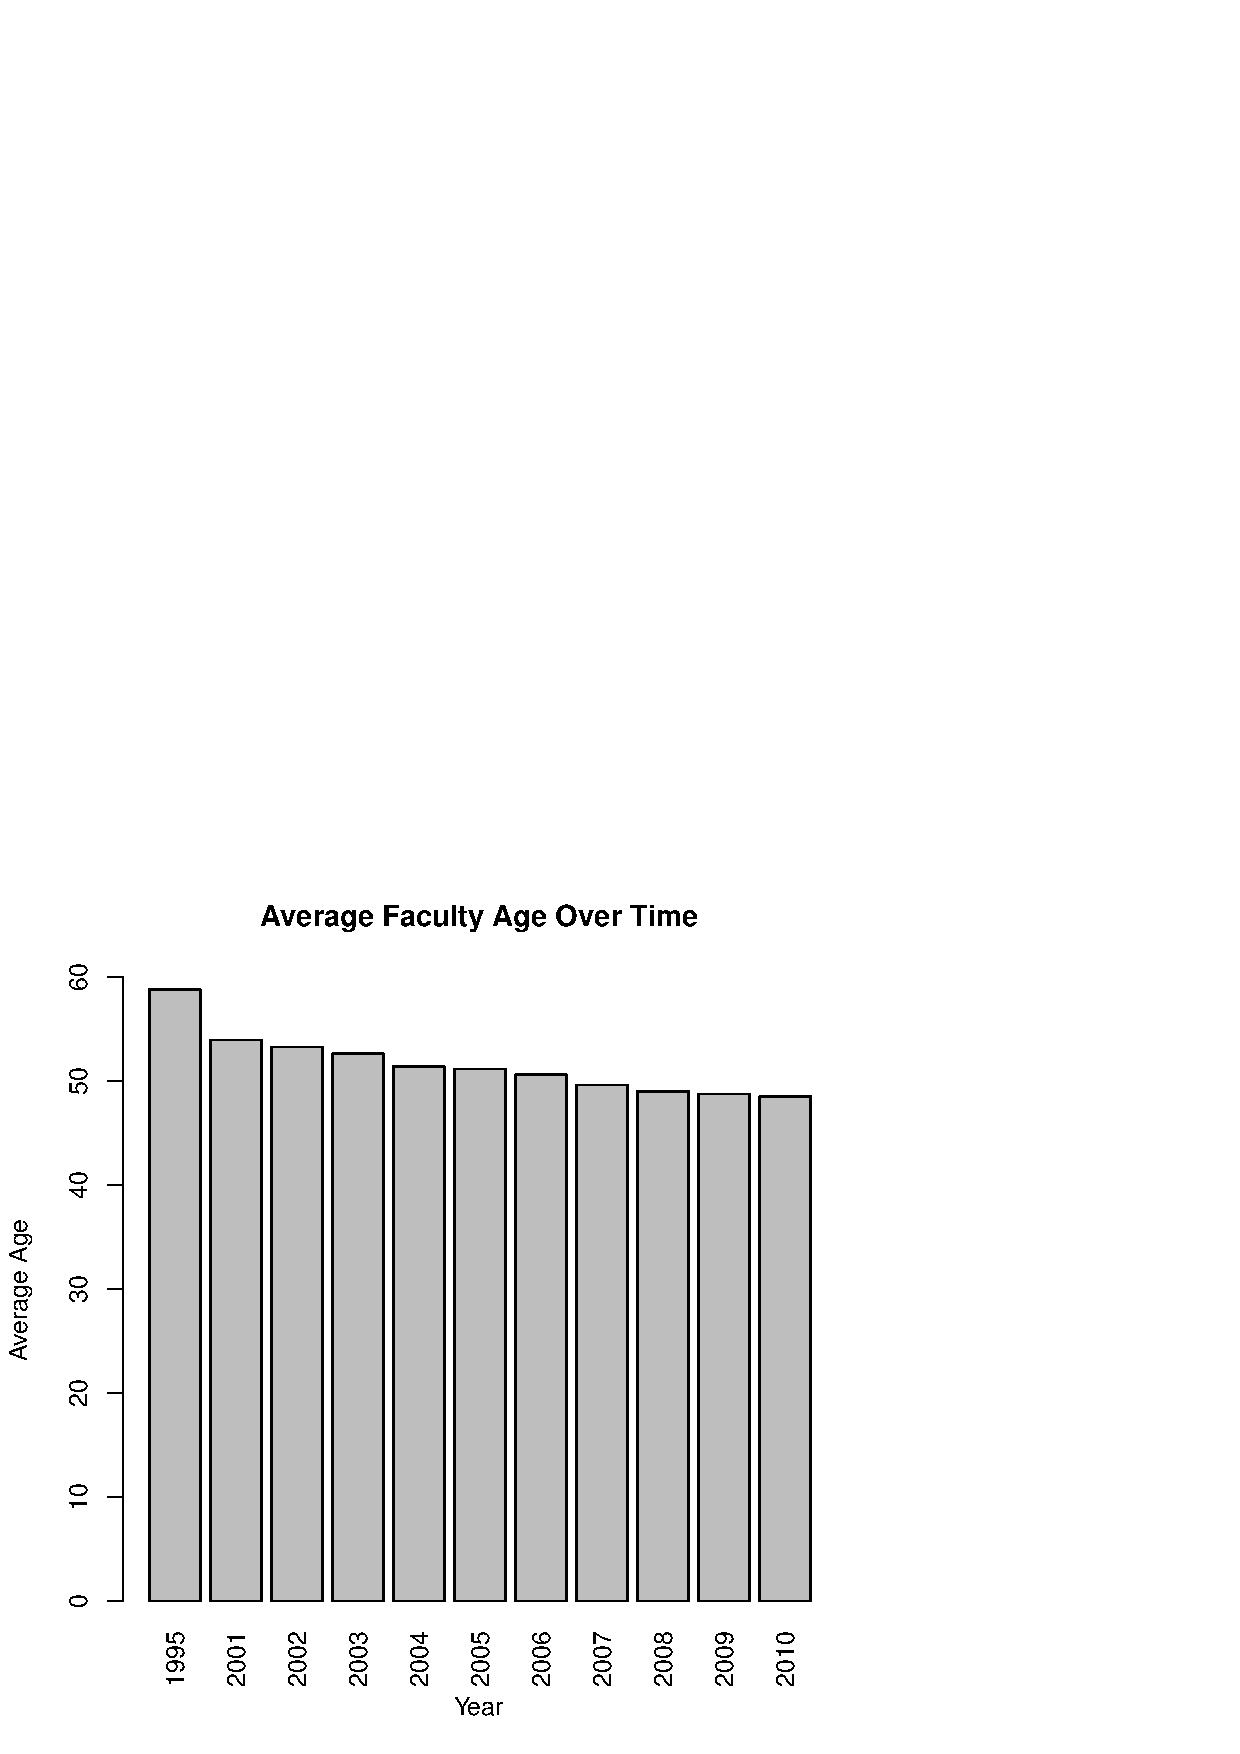
\includegraphics{faculty-003}
\caption{
The graph above plots the average age of all faculty members for each
academic year. The age is estimated by calculating the number number
of years since the faculty member received their undergraduate degree
and assuming an age of 22 at that time (age = 2010 - undergrad.year +
22). Unfortunately, not all the years of data provide degree
information, which explains the gap in the plot between 1995 and
2001. Furthermore, degree information was not provided for all faculty
members, so missing values were excluded as a result.
}

\end{figure}


\begin{figure}
  \centering
  \vspace*{.1in}
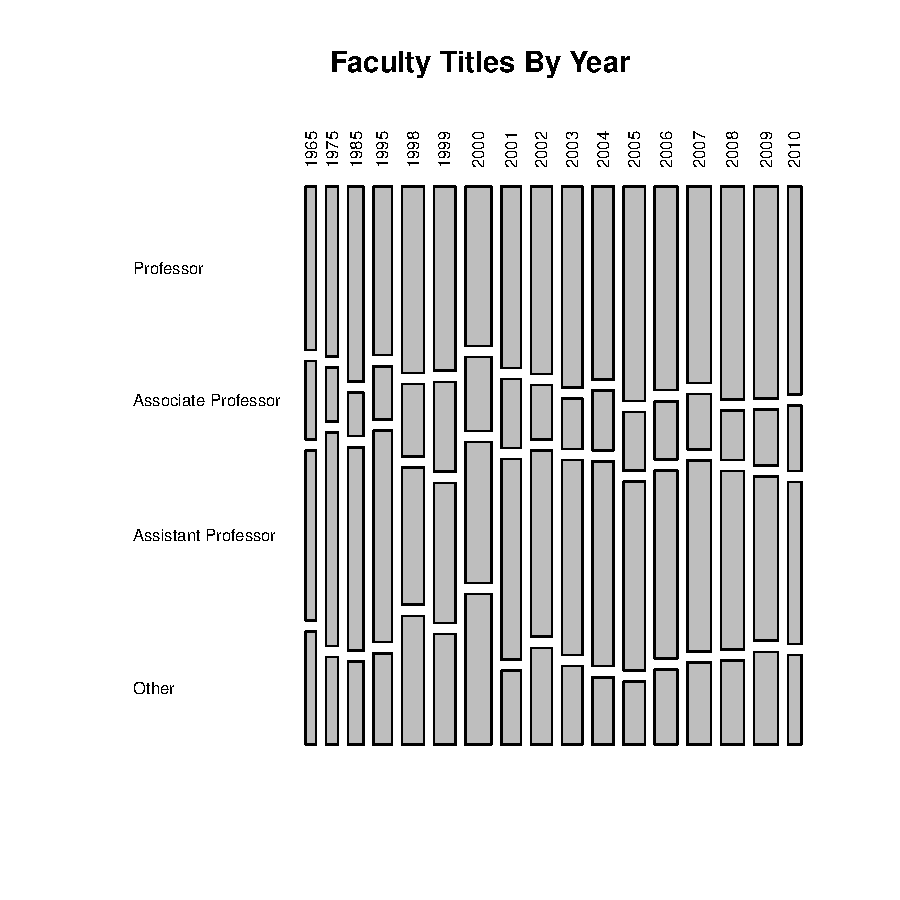
\includegraphics{faculty-005}

\caption{
The graph above plots the Williams College faculty titles over the
different academic years. The proportion of each title as a percentage
of the faculty for each academic year is easily comparable across
time, by comparing the vertical lengths of each bar. Furthermore, the
relative sizes of each year's faculty is represented by the width of
each bar, allowing us to compare overall faculty size across
time. Finally, both measures can be combined to compare the absolute
number of faculty within each title by comparing the areas of each bar.
}
\end{figure}

\address{Andrew Leeser \\
  Kane Capital Management \\
  Cambridge, MA, USA\\
  \email{aml05williams@yahoo.com}
}


\bibliography{orderbook}
\end{article}
\end{document}
